\section{实验环境}
\begin{itemize}
    \item 硬件环境：13th Gen Intel(R) Core(TM) i5-13420H 处理器，12 个逻辑处理器，主频约2.1 GHz；内存 16 GB。
    \item 软件环境：Windows、MacOS、WSL Arch Linux，Visual Studio Code 集成开发环境。
    \item 编程语言：Python 3.14。
    \item 求解与建模工具：Gurobi及其Python接口\texttt{gurobipy} 13.0.3、PyEDA 0.29.0（Espresso逻辑化简）、SageMath 10.9（凸包构造）。
    \item Python依赖管理：\texttt{uv}。
\end{itemize}
需要先安装Gurobi,免费的可以使用2000个变量和2000个约束条件,在这次实验里足够了
\begin{figure}[H]
    \centering
    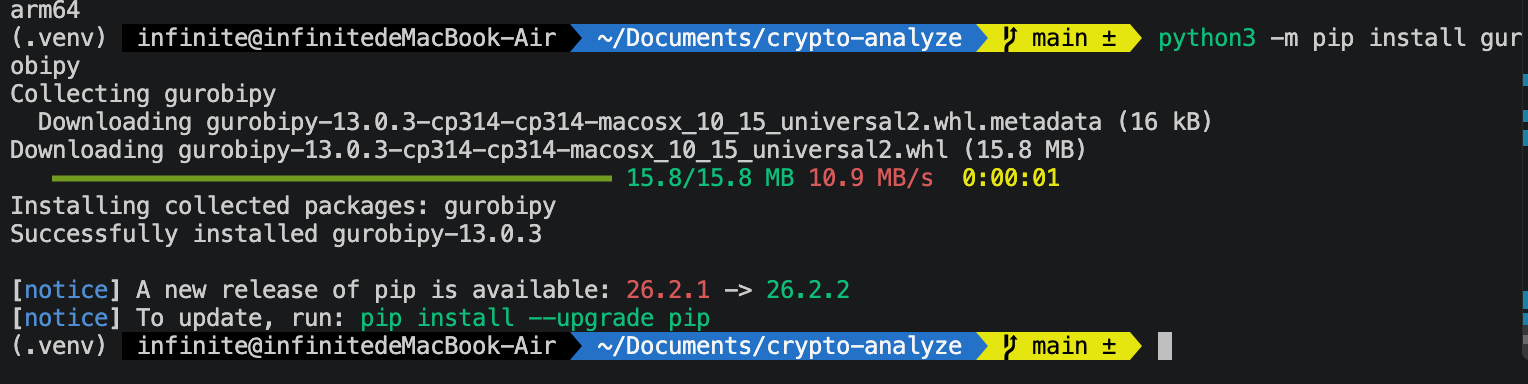
\includegraphics[width=0.8\textwidth]{figures/env.png}
    \caption{Gurobi安装界面}
    \label{fig:gurobi}
\end{figure}